\documentclass[a4paper,12pt,twoside]{scrreprt}
% Autor der Vorlage: Klaus Rheinberger, FH Vorarlberg
% 2017-02-20

%% Hilfe: z.B.
% empfohlener Einstieg: http://latex.tugraz.at/  
% https://de.wikibooks.org/wiki/LaTeX-Kompendium:_Schnellkurs:_Erste_Schritte
% https://de.wikibooks.org/wiki/LaTeX-Kompendium:_Schnellkurs
% https://de.wikibooks.org/wiki/LaTeX-Kompendium

%% Pakete:
% Der Befehl \usepackage[latin9]{inputenc} ermöglicht die direkte Angabe von Umlauten. Übrigens lässt sich so auch das Euro-Zeichen direkt eingeben. Auf Betriebssystemen, wie zum Beispiel allen neueren Linux-Distributionen, verwendet man statt \usepackage[latin9]{inputenc} besser \usepackage[utf8]{inputenc}, auf Applesystemen verwendet man \usepackage[macce]{inputenc} (oder das für ältere Modelle gültige \usepackage[applemac]{inputenc}).
\usepackage[utf8]{inputenc}
\usepackage[T1]{fontenc}    % Silbentrennung bei Sonderzeichen
\usepackage{graphicx}       % Bilder einbinden
\usepackage[british]{babel} % Deutsche Sprachanpassungen
\usepackage{csquotes}       % When using babel or polyglossia with biblatex, loading csquotes is recommended to ensure that quoted texts are typeset according to the rules of your main language.
\usepackage{acronym}  % für optionales Abkürzungsverzeichnis
\usepackage{eurosym}  % z. B. \EUR{12345,68}
\usepackage[linktocpage=true]{hyperref} % Links z. B. \href{https://www.wikibooks.org}{Wikibooks home}
\usepackage[bindingoffset=8mm]{geometry}% Bindeverlust von 8mm einbeziehen. Mit dem geometry-Paket können Sie die Ränder auch ganz individuell anpassen.
\usepackage{amsmath}
\usepackage{caption} % Abbildungslegenden
\usepackage{subcaption}
\usepackage{enumitem}

\usepackage{tabularx}
%\usepackage{biblatex}
%\usepackage[
%	backend=biber,
%	style=authoryear,
%]{biblatex}
\usepackage{algorithm}
\usepackage{algorithmic}
\captionsetup{format=hang, justification=raggedright}
\usepackage[style=alphabetic,citestyle=alphabetic,backend=biber]{biblatex}   % Literaturverweise
\usepackage{listings}
\usepackage{xcolor}

\colorlet{punct}{red!60!black}
\definecolor{background}{HTML}{EEEEEE}
\definecolor{delim}{RGB}{20,105,176}
\colorlet{numb}{magenta!60!black}

\lstdefinelanguage{json}{
	basicstyle=\normalfont\ttfamily,
	numbers=left,
	numberstyle=\scriptsize,
	stepnumber=1,
	numbersep=8pt,
	showstringspaces=false,
	breaklines=true,
	frame=lines,
	backgroundcolor=\color{background},
	literate=
	*{0}{{{\color{numb}0}}}{1}
	{1}{{{\color{numb}1}}}{1}
	{2}{{{\color{numb}2}}}{1}
	{3}{{{\color{numb}3}}}{1}
	{4}{{{\color{numb}4}}}{1}
	{5}{{{\color{numb}5}}}{1}
	{6}{{{\color{numb}6}}}{1}
	{7}{{{\color{numb}7}}}{1}
	{8}{{{\color{numb}8}}}{1}
	{9}{{{\color{numb}9}}}{1}
	{:}{{{\color{punct}{:}}}}{1}
	{,}{{{\color{punct}{,}}}}{1}
	{\{}{{{\color{delim}{\{}}}}{1}
	{\}}{{{\color{delim}{\}}}}}{1}
	{[}{{{\color{delim}{[}}}}{1}
	{]}{{{\color{delim}{]}}}}{1},
}

%\usepackage[style=numeric,citestyle=numeric,backend=biber]{biblatex}
% biblatex comes with a variety of built-in bibliography/citation style families (numeric, alphabetic, authoryear, authortitle, verbose), and there's a growing number of custom styles:
% https://de.sharelatex.com/learn/Biblatex_citation_styles
% https://de.sharelatex.com/learn/Biblatex_bibliography_styles
\addbibresource{ma.bib}    % Zotero-Beispiele.bib ist die verwendete Bibtex-Datei 
% Anstatt die Bibtex-Datei selber zu erstellen, kann sie z. B. aus einer Zotero-Sammlung zu BibTeX exportiert werden.
\DeclareCaptionFormat{algor}{%
	\hrulefill\par\offinterlineskip\vskip1pt%
	\textbf{#1#2}#3\offinterlineskip\hrulefill}
\DeclareCaptionStyle{algori}{singlelinecheck=off,format=algor,labelsep=space}

%% Einstellungen:
\usepackage{chngcntr}
\counterwithout{equation}{chapter}
\setcounter{secnumdepth}{4}
\setcounter{equation}{0}
\setcounter{tocdepth}{4}   % Tiefe der Gliederung im In haltsverzeichnis
\nocite{*}
%% ERSETZEN VON ECKIGEN KLAMMERN:
% Ersetzen Sie den Text in den eckigen Klammern!

\begin{document}


% Titelblatt:
% \newpage\mbox{}\newpage
\cleardoublepage   % force output to a right page
\thispagestyle{empty}
\begin{titlepage}
  \begin{flushleft}
  \section*{Modell für Scheduling}
  
  \end{flushleft}
\end{titlepage}

% Kurzreferat:
\newpage
\section*{Benötigte Daten}
\subsection*{Beschreibung}
Die Daten sind in 2 Teile aufgeteilt:
\begin{itemize}
	\item System-Info, beinhaltet Informationen über die Umgebung in der produziert wird
	\item Orders, beinhaltet Kundenaufträge/Bestellungen, die in dem beschriebenen System umgesetzt werden sollen
\end{itemize}
\subsubsection*{System-Info}
Beinhaltet Informationen über die Produktions-Umgebung
\paragraph*{Tasks}
Alle Arbeitsschritte / Aktionen, die in der Produktions-Umgebung durchgeführt werden können.
(Wichtig: Tasks die z.Bsp. bei Task A als „follow up task“ angegeben werden sollen KEINEN Verweis auf Task A in den „preciding tasks“ haben). Die zeitliche Dauer jedes Tasks ist bei den Workstations( \autoref{workstation}) abgebildet, um die Umsetzung einer Aufgabe mit verschiedenen Maschinen/Werkzeugen zu berücksichtigen.
\begin{itemize}
	\item id – eindeutige ID des Tasks (kann fortlaufende Nummer sein, nur für interne Identifizierung)
	\item name – Name des Tasks (für einfacher lesbare Ergebnisse)
	\item resources – (liste) benötigt Ressourcen, um den Task durchzuführen (id + anzahl)
	\item products – (liste) alle Ressourcen (ID + Anzahl (Losgröße)) die durch den Task entstehen
	\item preceding\_tasks – (liste) Tasks, die gemeinsam mit diesem Task durchgeführt werden müssen (vorangestellte Tasks, müssen daher nicht extra als Arbeitsschritt übermittelt werden)
	\item follow\_up\_tasks – (liste) Tasks, die nach dem Task durchgeführt werden müssen (wie preciding tasks)
	\item independent – boolean, um festzustellen, ob der Task im Schedule verwendet werden soll (e.g. false für Tasks die immer nur als vorangestellter Task vorkommen und allein keinen Sinn ergeben)
	\item prepare\_time – Zeit die zum Einrichten der Maschine/Arbeitsstation für diesen Task benötigt wird
	\item unpreprare\_time – Zeit, die nach der Verwendung der Maschine/Arbeitsstation für diesen Task benötigt wird
\end{itemize}
\paragraph*{Recipes}
Die Rezepte für die verschiedenen Ressourcen, die hergestellt werden sollen (Produkte oder auch Zwischenprodukte)
\begin{itemize}
	\item id – eindeutige ID des Rezepts (kann auch fortlaufende Nummer sein, nur für interne Identifizierung)
	\item name – Name des Rezepts (für einfacher lesbare Ergebnisse)
	\item tasks – (liste) IDs der Tasks, die durchgeführt werden müssen, um das Rezept umzusetzen (Ergebnis und Ergebnismenge ergeben sich aus dem letzten Task)
\end{itemize}
\paragraph*{Resources}
Alle Ressourcen, die in der Produktions-Umgebung verwendet oder hergestellt werden können
\begin{itemize}
	\item id – eindeutige ID der Ressource (kann auch fortlaufende Nummer sein, nur für interne Identifizierung)
	\item name – Name der Ressource (für einfacher lesbare Ergebnisse)
	\item stock – Anzahl der Ressource im Lagerbestand
	\item price – Preis pro Einheit, um die Ressource einzukaufen (0 wenn die Ressource nicht gekauft werden kann)
	\item delivery\_time - Erwartete Wartezeit, falls die Ressource eingekauft werden muss
	\item renewable – boolean, um festzustellen, ob die Ressource verbraucht wird oder nicht (könnte z.Bsp. auch Ressource Mitarbeiter sein, der wieder verfügbar ist, wenn ein Task beendet ist)
	\item recipes – (liste) IDs der Rezepte, durch die diese Ressource hergestellt werden kann (falls vorhanden, sonst leere Liste)
\end{itemize}
\paragraph*{Workstations}
\label{workstation}
Alle Maschinen / Arbeitsstationen, die in der Produktions-Umgebung vorhanden sind
\begin{itemize}
	\item id – eindeutige ID der Maschine/Arbeitsstation (kann auch fortlaufende Nummer sein, nur für interne Identifizierung)
	\item name – Name der Maschine/Arbeitsstation (für einfacher lesbare Ergebnisse)
	\item basic\_resources – (liste) beinhaltet die IDs der benötigten Ressourcen + die Anzahl für jede Ressource, die (unabhängig der bevorstehenden Tasks) benötigt werden um die Maschine/Arbeitsstation zu betreiben (z.Bsp. Mitarbeiter)
	\item tasks – (liste) IDs aller Tasks, die auf dieser Maschine/Arbeitsstation durchgeführt werden können + die Dauer des Tasks auf dieser Maschine/Arbeitsstation
\end{itemize}

\subsubsection*{Orders}
Repräsentiert Kundenaufträge/Bestellungen, die mithilfe der Produktions-Umgebung umgesetzt werden soll.
\begin{itemize}
	\item id – eindeutige ID der Bestellung (kann auch fortlaufende Nummer sein, nur für interne Identifizierung)
	\item arrival\_time – Zeitpunkt, zu dem die Bestellung im System eingegangen ist
	\item delivery\_time – Zeitpunkt, zu dem die Bestellung fertig sein soll
	\item latest\_acceptable\_time – Spätester Zeitpunkt, zu dem die Bestellung fertig sein soll, 
	falls der gewünschte Lieferzeitpunkt nicht eingehalten kann
	\item resources – (liste) IDs + Anzahl der bestellten Ressourcen, die hergestellt werden sollen, + der Preis, den der Kunde für diese Ressource bezahlen wird
	\item penalty – falls die Bestellung nicht durchgeführt wird
	\item tardiness\_fee – falls die Bestellung nach dem gewünschten Termin, aber vor dem letzten möglichen Termin durchgeführt wird
	\item divisible – boolean, gibt an ob auch nur Teile der Bestellung bearbeitet werden können, oder ob alle bestellten Ressourcen geliefert werden müssen (oder gar keine)
	\item customer\_id – ID des Kunden, von dem der Auftrag stammt
	\item optional - boolean, gibt an ob eine Bestellung zwingend im Schedule vorhanden sein muss oder nicht (default: true)
\end{itemize}

\subsection*{Jobs}
Repräsentiert die spezifische Ausführung eines Tasks für eine Bestellung
\begin{itemize}
	\item id - eindeutige ID des Jobs (kann auch fortlaufende Nummer sein, nur für interne Identifizierung)
	\item order\_id - ID der Bestellung, für die der Job ausgeführt werden muss
	\item task\_id - ID des Tasks, der ausgeführt werden soll
	\item to\_id - Spezifische Zuteilungs-ID zwischen Tasks und Bestellungen, um den Job im Schedule genau zuordnen zu können
\end{itemize}

\begin{figure}[H]
	\centering
	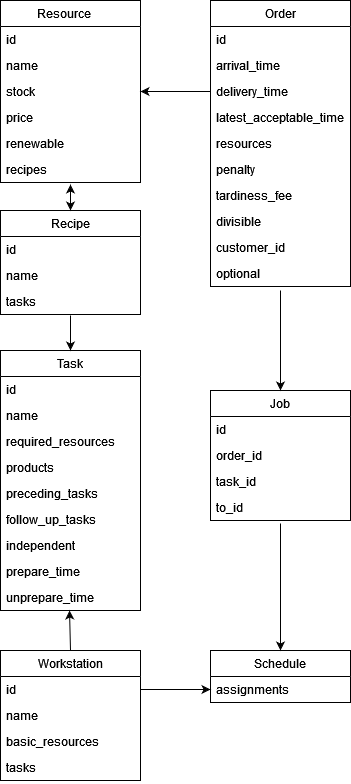
\includegraphics[width=8cm]{images/dependencies_v2}
	\caption{Dependencies}
	\label{fig:dependencies}
\end{figure}

\section*{Input / Output}
Genaue Struktur der Datenübertragung mit Beispieldaten unter "JSON-Beispiel"(\autoref{json_example})
\begin{flushleft}
	Input:\linebreak
	Orders:\linebreak
	$Order A$\linebreak
	$Task_1 - Task_n$\linebreak
	$price_1 - price_n$\linebreak
	$penalty$\linebreak
	$tardiness\_fee$\linebreak
	$delivery\_date$\linebreak
	$latest\_date$\linebreak
	$optional$\linebreak
	
	Mapping von Tasks zu Jobs Bsp.:\linebreak
	(Zuteilung zu exakten Job, Bsp. Task: Material schneiden -> Job: Material schneiden für Bestellung A)\linebreak
	$Task A.1$\linebreak
	$Task ID$\linebreak
	$Job ID$ \linebreak\linebreak
	Intermediate:\linebreak
	<Workstation ID, Task (Operation) ID, Start Time Slot>
	$j_1 - (w, t, s)$\linebreak
	$j_2 - (w, t, s)$\linebreak
	$j_2 - (w, t, s)$\linebreak
	.\linebreak
	.\linebreak
	.\linebreak
	$j_n - (w, t, s)$\linebreak\linebreak
	Output:\linebreak
	$
	\begin{bmatrix}
		(j_{11}, s_{11}) & (j_{12}, s_{12}) & (j_{13}, s_{13}) & \dots & (j_{1n}, s_{1n})\\
		(j_{21}, s_{21}) & (j_{22}, s_{22}) & (j_{23}, s_{23}) & \dots & (j_{2n}, s_{2n})\\
		\hdotsfor{5} \\
		(j_{m1}, s_{m1}) & (j_{m2}, s_{m2}) & (j_{m3}, s_{m3}) & \dots & (j_{mn}, s_{mn})\\
	\end{bmatrix}
	$
	
	\begin{figure}[H]
		\centering
		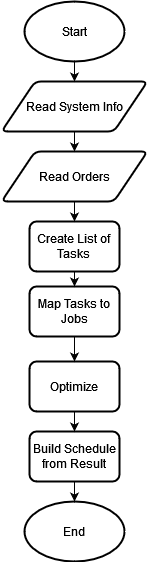
\includegraphics[width=4cm]{images/ablauf}
		\caption{Ablauf}
		\label{fig:ablauf}
	\end{figure}
\end{flushleft}
\section*{Modell}
\subsection*{Variablen Definition}
\begin{flushleft}
OLD: \linebreak
$O$ - Set of all Orders\linebreak
$o$ - Specific Order, $o \in O$\linebreak
$W$	- Set of all Workstations\linebreak
$T$	- Set of all Tasks\linebreak
$T_{o}$ - Set of all Tasks needed for Order $o$, $T_{o} \subset T$\linebreak
$x$ - Specific Task, $x \in T$\linebreak
$T_{xp}$ - Set of all Tasks preceding Task $x$, $T_{xp} \subset T$\linebreak
$T_{xf}$ - Set of all Tasks following Task $x$, $T_{xf} \subset T$\linebreak
$J$ - Set of all Jobs\linebreak
$J_{w}$ - Set of all Jobs assigned to Workstation $w$, $w \in W$\linebreak
$j_{x}$ - Job linked to Task $j$, $x \in T$, $j \in J$\linebreak
$x_{j}$ - Task linked to Job $j$, $x \in T$, $j \in J$\linebreak
$W_{j}$ -	Set of Workstations eligible for Job $j$, $W_{j}$ $\subset$ $W$ \linebreak
$R$ - Set of all Resources \linebreak
$w$ - Specific Workstation $w \in W$ \linebreak
$R_{j}$ - Set of Resources needed for Job $j$, $R_{j} \subset$ $R$ \linebreak
$r$ - Specific Resource, $r \in R$ \linebreak
$d_{xw}$ - Duration of Task $x$ on Workstation $w$ \linebreak
$j_{w}$ - Selected Workstation for a Job $j$, $w\in W_{j}$ \linebreak
$j_{s}$ - Start time slot of Job $j$\linebreak
$j_{dt}$ - Deliver time slot of Job $j$\linebreak
$j_{lt}$ - Latest allowed time slot of Job $j$\linebreak
$i_{rt}$ - Amount of Resource $r$ in the Inventory at time slot $t$\linebreak
$l_{j}$ - Binary Variable, 1 if Job $j$ is late (Tardiness Fee applies)\linebreak
$l_{o}$ - Binary Variable, 1 if Order $o$ is late (Tardiness Fee applies)\linebreak
$u_{o}$ - Binary Variable, 1 if Order $o$ can only be fulfilled partially\linebreak
$p_{o}$ - Price the customer pays for Order $o$ \linebreak
$f_{o}$ - Price reduction for tardy orders \linebreak
$O_{c}$ - Set of all Orders which could be completed in the derived schedule, $O_{c} \subset O$\linebreak

NEW SUGGESTION: \linebreak
$O$ - Set of all Orders \linebreak
$P$ - Set of all Tasks \linebreak
$W$ - Set of all Workstations \linebreak
$R$ - Set of all Resources \linebreak
$X$ - Set of all Jobs \linebreak
$o$ - Specific Order, $o \in O$\linebreak
$p$ - Specific Task, $p \in P$\linebreak
$w$ - Specific Workstation $w \in W$ \linebreak
$r$ - Specific Resource, $r \in R$ \linebreak
$x$ - Specific Job, $x \in X$ \linebreak
$P_{o}$ - Set of all Tasks needed to complete Order $o$, $P_{o} \subset P$ \linebreak
$P_{p_{pre}}$ - Set of all Tasks preceding Task $p$, $P_{p_{pre}} \subset P$ \linebreak
$P_{p_f}$ - Set of all Tasks following Task $p$, $P_{p_{f}} \subset p$ \linebreak
$X_{w}$ - Set of all Jobs assigned to Workstation $w$, $w \in W$, $X_{w} \subset X$ \linebreak
$W_{x}$ - Set of all Workstations eligible for Job $x$, $x \in X$, $W_{x} \subset W$ \linebreak
$R_{x}$ - Set of all Resources required for Job $x$, $x \in X$, $R_{x} \subset R$ \linebreak
$d_{pw}$ - Duration of Task $p$ on Workstation $w$, $p \in P$, $w \in W$, $d_{pw} \geq 0$ \linebreak
$x_{w}$ - Selected Workstation $w$ for Job $x$, $x \in X$, $w \in W$, $x_{w} \in W$ \linebreak
$x_{s}$ - Start time slot for Job $x$, $x \in X$, $x_{s} \geq 0$ \linebreak
$x_{p}$ - Task $p$ corresponding to Job $x$, $x \in X$, $p \in P$, $x_{p} \in X$ \linebreak
$x_{dt}$ - Delivery time slot for Job $x$, $x \in X$, $x_{dt} \geq 0$ \linebreak
$x_{lt}$ - Latest acceptable time slot for Job $x$, $x \in X$, $x_{lt} \geq 0$, $x_{lt} \geq x_{dt}$ \linebreak
$a_{r,t}$ - Amount of Resource $r$ in stock at time slot $t$, $r \in R$, $t \geq 0$, $a_{r,t} \geq 0$ \linebreak
$l_{x}$ - Binary Variable, 1 if Job $x$ is late (Tardiness Fee applies), $x \in X$ \linebreak
$l_{o}$ - Binary Variable, 1 if Order $o$ is late (Tardiness Fee applies), $o \in O$ \linebreak
$u_{o}$ - Binary Variable, 1 if Order $o$ can only be fulfilled partially, $o \in O$, \linebreak
$z_{o}$ - Price the customer pay for Order $o$, $o \in O$, $z_{o} \geq 0$ \linebreak
$f_{o}$ - Price reduction for tardy orders , $o \in O$, $f_{o} \geq 0$ \linebreak
$o_{opt}$ - Binary Variable, 1 if Order $o$ is optional, $o \in O$ \linebreak
$o_{lt}$ - Latest acceptable time for Order $o$, $o \in O$, $lt \geq 0$ \linebreak
$b_{o}$ - Penalty, if Order $o$ is not scheduled to meet $o_{lt}$, $o \in O$, $b \geq 0$ \linebreak
$O_{c}$ - Set of all Orders which could be completed in the schedule, $O_{c} \subset O$ \linebreak


\end{flushleft}

\subsection*{Objective Function + Nebenbedingungen}
\subsubsection*{Objective Functions}
\begin{flushleft}
\autoref{objective_function_1} Minimize tardy jobs\linebreak
\autoref{objective_function_2} Maximize earning\linebreak
\autoref{objective_function_3} Minimize deviation from the expected delivery date\linebreak
\autoref{objective_function_4} Maximize Set Size of scheduled jobs\linebreak
\autoref{objective_function_5} Maximize Set Size of scheduled jobs with least tardy jobs\linebreak
\autoref{objective_function_6} Maximize Set Size of scheduled jobs with least deviations\linebreak
	\begin{equation}
	\label{objective_function_1}
	\begin{split}
		X := X_{i} \\
		minimize \sum_{i=0}^{X}l_{x} 
	\end{split}
	\end{equation}
	\begin{equation}
	\label{objective_function_2}
	\begin{split}
		o := O_{c,i} \\
		maximize \sum_{i=0}^{O_{c}}p_{o} - (l_{o} * f_{o})
	\end{split}
	\end{equation}
	\begin{equation}
	\label{objective_function_3}
	\begin{split}
		x := X_{i} \\
		y := p_{j} \\
		minimize \sum_{i=0}^{X} |(x_{s} + d_{y,w}) - x_{dt}|
	\end{split}
	\end{equation}
	\begin{equation}
	\label{objective_function_4}
	\begin{split}
		maximize |O_{c}|
	\end{split}
	\end{equation}
	\begin{equation}
	\label{objective_function_5}
	\begin{split}
		x := X_{i} \\
		maximize |O_{c}| - \sum_{i=0}^{X}l_{x}
	\end{split}
	\end{equation}
	\begin{equation}
	\label{objective_function_6}
	\begin{split}
		x := X_{i} \\
		y := p_{x} \\
		z ... threshold for acceptable deviation \\
		d := \sum_{i=0}^{X} (|(x_{s} + d_{y,w}) - x_{dt}| > z)\\
		maximize |O_{c}| - d
	\end{split}
	\end{equation}
\end{flushleft}
\subsubsection*{Nebenbedingungen}
\begin{flushleft}
\autoref{not_late} to make sure jobs finish before last possible time slot\linebreak
\autoref{sufficient_resources} to make sure jobs have sufficient resources to start\linebreak
\autoref{check_tardiness} checks if tardiness fee applies\linebreak
\autoref{no_early_start} jobs can't start before preceding tasks finish\linebreak
\autoref{follow_up_tasks_early_start} follow up jobs can't start before job finished\linebreak
\autoref{no_multiple_workstation_occupations} only one active job at one time slot for each Workstation\linebreak
\autoref{only_legal_timeslots} starting times need to be after timeslot 0\linebreak
\end{flushleft}

\begin{flushleft}
	UPDATED:\linebreak
	\begin{equation}
	\label{not_late}
		x_{s} \leq x_{lt} - d_{x_{p}, x_{w}}
	\end{equation}
	\begin{equation}
		\label{check_tardiness}
		\begin{split}
			l_{x} := x_{dt} \leq x_{s} \leq x_{lt} \\
		\end{split}
	\end{equation}
	\begin{equation}
	\label{only_legal_timeslots}
	\begin{split}
		x := X_{i} \\
		\sum_{i=0}^{X} (x_{s} < 0) < 1
	\end{split}
	\end{equation}
	\begin{equation}
	\label{sufficient_resources}
	\begin{split}
		r := R_{xi} \\
		\sum_{i=0}^{R_{x}}(a_{r,t}-r\leq 0) < 1\\
	\end{split}
	\end{equation}
	\begin{equation}
	\label{no_early_start}
	\begin{split}
		y := P_{x_{p}pre, i} \\
		y' := P_{x_{p}pre, i-1} \\
		z := \sum_{i=1}^{P_{x_{p}pre}} (x_{ys} + d_{yw}) - (x_{y'} + d_{y'w}) < 0 \\
		z < 1 \\
	\end{split}
	\end{equation}
	\begin{equation}
	\label{follow_up_tasks_early_start}
	\begin{split}
		y := P_{x_{p}f, i}\\
		y' := P_{x_{p}f, i-1}\\
		z := \sum_{i=1}^{P_{x_{p}f}} (x_{y's} + d_{y'w}) < x_{ys}\\
		z < 1
	\end{split}
	\end{equation}
	NOT YET UPDATED:\linebreak
	\begin{equation}
	\label{no_multiple_workstation_occupations}
	\begin{split}
		\forall w \in W \\
		i = J_{wm} \\
		j = J_{wn} \\
		x = x_{i} \\
		x' = x_{j} \\
		\sum_{m=0}^{J_{w}} (\sum_{n = 0}^{J_{w}-1}((1-(j_{s} + d_{x',w} < i_{s})) + (1-(j_{s} > i_{s} + d_{x,w})))) < 1
	\end{split}
	\end{equation}

\end{flushleft}
\section*{JSON-Beispiel}
\label{json_example}
\begin{lstlisting}[language=json,firstnumber=1]
{
"system-info":
	{
	"tasks":
	[
		{
			"id": 0,
			"name": "Task 1",
			"resources":
			[
				{
					"id": 0,
					"amount": 10
				}
			],
			"products":
			[
				{
					"resource_id": 1,
					"amount": 1
				}
			],
			"preceding_tasks":
			[],
			"follow_up_tasks":
			[
				1
			],
			"independent": true,
			"prepare_time": 5,
			"unprepare_time": 5
		},
		{
			"id": 1,
			"name": "Task 2",
			"resources":
			[
				{
					"id": 1,
					"amount": 1
				}
			],
			"products":
			[
				{
					"resource_id": 2,
					"amount": 1
				}
			],
			"preceding_tasks":
			[],
			"follow_up_tasks":
			[],
			"independent": false,
			"prepare_time": 0,
			"unprepare_time": 5
		},
		{
			"id": 2,
			"name": "Task 3",
			"resources":
			[
				{
					"id": 3,
					"amount": 20
				},
				{
					"id": 4,
					"amount": 10
				}
			],
			"products":
			[
				{
					"resource_id": 5,
					"amount": 2
				},
				{
					"resource_id": 6,
					"amount": 1
				}
			],
			"preceding_tasks":
			[
				3, 4
			],
			"follow_up_tasks":
			[],
			"independent": true,
			"prepare_time": 10,
			"unprepare_time": 5
		},
		{
			"id": 3,
			"name": "Task 4",
			"resources": 
			[
				{
					"id": 7,
					"amount": 5
				}
			],
			"products":
			[
				{
					"resource_id": 3,
					"amount": 20
				}
			],
			"preceding_tasks":
			[],
			"follow_up_tasks":
			[],
			"independent": false,
			"prepare_time": 5,
			"unprepare_time": 5
		},
		{
			"id": 4,
			"name": "Task 5",
			"resources":
			[
				{
					"id": 8,
					"amount": 1
				}
			],
			"products":
			[
				{
					"resource_id": 4,
					"amount": 5
				}                
			],
			"preceding_tasks":
			[],
			"follow_up_tasks":
			[],
			"independent": true,
			"prepare_time": 1,
			"unprepare_time": 5
		},
		{
			"id": 5,
			"name": "Task 6",
			"resources":
			[
				{
					"id": 9,
					"amount": 20
				},
				{
					"id": 10,
					"amount": 1
				}
			],
			"products":
			[
				{
					"resource_id": 8,
					"amount": 2
				}
			],
			"independent": true,
			"preceding_tasks":
			[],
			"follow_up_tasks":
			[],
			"prepare_time": 5,
			"unprepare_time": 5
		}
	],
	"recipes":
	[
		{
			"id": 0,
			"name": "Recipe 1",
			"tasks":
			[
				5
			]
		},
		{
			"id": 1,
			"name": "Recipe 2",
			"tasks":
			[
				2
			]
		},
		{
			"id": 2,
			"name": "Recipe 3",
			"tasks":
			[
				0
			]
		},
		{
			"id": 3,
			"name": "Recipe 4",
			"tasks":
			[
				4
			]
		}
		],
	"resources":
	[
		{
			"id": 0,
			"name": "Resource 1",
			"stock": 50,
			"price": 20,
			"delivery_delay": 0,
			"renewable": false,
			"recipes":
			[]
		},
		{
			"id": 1,
			"name": "Resource 2",
			"stock": 0,
			"price": 300,
			"delivery_delay": 0,
			"renewable": false,
			"recipes":
			[]
		},
		{
			"id": 2,
			"name": "Resource 3",
			"stock": 10,
			"price": 1000,
			"delivery_delay": 0,
			"renewable": false,
			"recipes":
			[
				2
			]
		},
		{
			"id": 3,
			"name": "Resource 4",
			"stock": 100,
			"price": 10,
			"delivery_delay": 0,
			"renewable": false,
			"recipes":
			[]
		},
		{
			"id": 4,
			"name": "Resource 5",
			"stock": 10,
			"price": 100,
			"delivery_delay": 0,
			"renewable": false,
			"recipes":
			[
				3
			]
		},
		{
			"id": 5,
			"name": "Resource 6",
			"stock": 4,
			"price": 50,
			"delivery_delay": 0,
			"renewable": false,
			"recipes":
			[
				1
			]
		},
		{
			"id": 6,
			"name": "Resource 7",
			"stock": 3,
			"price": 70,
			"delivery_delay": 0,
			"renewable": false,
			"recipes":
			[
				1
			]
			},
		{
			"id": 7,
			"name": "Resource 8",
			"stock": 15,
			"price": 15,
			"delivery_delay": 0,
			"renewable": false,
			"recipes":
			[]
		},
		{
			"id": 8,
			"name": "Resource 9",
			"stock": 6,
			"price": 700,
			"delivery_delay": 0,
			"renewable": false,
			"recipes":
			[
				0
			]
		},
		{
			"id": 9,
			"name": "Resource 10",
			"stock": 40,
			"price": 200,
			"delivery_delay": 0,
			"renewable": false,
			"recipes":
			[]
		},
		{
			"id": 10,
			"name": "Resource 11 (Employee)",
			"stock": 10,
			"price": 0,
			"delivery_delay": 0,
			"renewable": true,
			"recipes":
			[]
		},
		{
			"id": 11,
			"name": "Resource 12",
			"stock": 1000,
			"price": 5,
			"delivery_delay": 0,
			"renewable": false,
			"recipes":
			[]
		}
	],
	"workstations":
	[
		{
			"id": 0,
			"name": "Workstation 1",
			"basic_resources":
			[
				{
					"id": 10,
					"amount": 1
				}
			],
			"tasks":
			[
				{
					"task_id": 0,
					"duration": 10
				},
				{
					"task_id": 2,
					"duration": 5
				}
			]
		},
		{
			"id": 1,
			"name": "Workstation 2",
			"basic_resources":
			[
				{
					"id": 10,
					"amount": 1
				},
				{
					"id": 11,
					"amount": 2
				}
			],
			"tasks":
			[
				{
					"task_id": 1,
					"duration": 20
				},
				{
					"task_id": 2,
					"duration": 7
				}
			]
		},
		{
			"id": 2,
			"name": "Workstation 3",
			"basic_resources":
			[],
			"tasks":
			[
				{
					"task_id": 3,
					"duration": 1
				},
				{
					"task_id": 4,
					"duration": 2
				},
				{
					"task_id": 5,
					"duration": 15
				}
			]
		},
		{
			"id": 3,
			"name": "Workstation 4",
			"basic_resources":
			[
				{
					"id": 10,
					"amount": 1
				}
			],
			"tasks":
			[
				{
					"task_id": 4,
					"duration": 1
				},
				{
					"task_id": 5,
					"duration": 10
				}
			]
		}
	]
},
"orders":
[
	{
		"id": 0,
		"arrival_time": "2022-02-07 00:00:00",
		"delivery_time": "2022-02-20 14:30:00",
		"latest_acceptable_time": "2022-02-22 00:00:00",
		"resources":
		[
			{
				"id": 2,
				"amount": 5,
				"price": 700
			},
			{
				"id": 4,
				"amount": 10,
				"price": 300
			}
		],
		"penalty": 300,
		"tardiness_fee": 100,
		"divisible": false,
		"customer_id": 1,
		"optional": true
	},
	{
		"id": 1,
		"arrival_time": "2022-02-17 00:00:00",
		"delivery_time": "2022-02-21 15:30:00",
		"latest_acceptable_time": "2022-02-24 00:00:00",
		"resources":
		[
			{
				"id": 4,
				"amount": 20,
				"price": 600
			},
			{
				"id": 5,
				"amount": 10,
				"price": 2000
			}
		],
		"penalty": 500,
		"tardiness_fee": 100,
		"divisible": false,
		"customer_id": 1,
		"optional": true
	},
	{
		"id": 2,
		"arrival_time": "2022-02-10 00:00:00",
		"delivery_time": "2022-02-19 14:00:00",
		"latest_acceptable_time": "2022-02-26 00:00:00",
		"resources":
		[
			{
				"id": 2,
				"amount": 20,
				"price": 2700
			},
			{
				"id": 5,
				"amount": 10,
				"price": 2000
			}
		],
		"penalty": 1000,
		"tardiness_fee": 100,
		"divisible": false,
		"customer_id": 1,
		"optional": true
	},
	{
		"id": 3,
		"arrival_time": "2022-02-08 00:00:00",
		"delivery_time": "2022-02-23 17:00:00",
		"latest_acceptable_time": "2022-02-26 00:00:00",
		"resources":
		[
			{
				"id": 5,
				"amount": 17,
				"price": 3500
			},
			{
				"id": 6,
				"amount": 10,
				"price": 1200
			}
		],
		"penalty": 700,
		"tardiness_fee": 200,
		"divisible": false,
		"customer_id": 1,
		"optional": true
	},
	{
		"id": 4,
		"arrival_time": "2022-02-15 00:00:00",
		"delivery_time": "2022-02-23 12:00:00",
		"latest_acceptable_time": "2022-02-26 00:00:00",
		"resources":
		[
			{
				"id": 4,
				"amount": 34,
				"price": 800
			},
			{
				"id": 8,
				"amount": 10,
				"price": 3000
			}
		],
		"penalty": 200,
		"tardiness_fee": 100,
		"divisible": false,
		"customer_id": 1,
		"optional": true
	}
]
}
\end{lstlisting}
\end{document}
